%=====================================================================
\section{Active circles: where the defects sit}\label{sec:cdist}
\subsection{Maps and profiles across sizes}
Figure~\ref{fig:maps-circ} shows the time-averaged defect density of active circles with $k=6$ and five radii,
$R=0.57$, 0.86, 1.43, 2.15 and $2.87\,\la$ (main sweep, seed 1, $\zeta=0.07$), together with one passive circle of $k=6$ at
$R=1.43\,\la$. Because $k$ is fixed, the imposed density $\rho=k/(\pi R)$ falls as the cavity grows (0.15, 0.10, 0.06, 0.04,
0.03), so this series changes size and density together; the dependence on $k$ at fixed size is in Sec.~\ref{sec:cdist-k}, and the full
$(\rho,R/\la)$ plane in Sec.~\ref{sec:sweep}. Figure~\ref{fig:prof-circ} gives, for the same runs, the $+\half$ and $-\half$
densities and the $+\half$ speed against the distance from the wall in units of $\la$ (method: Sec.~\ref{sec:m-dist}).

\begin{figure}[H]\centering
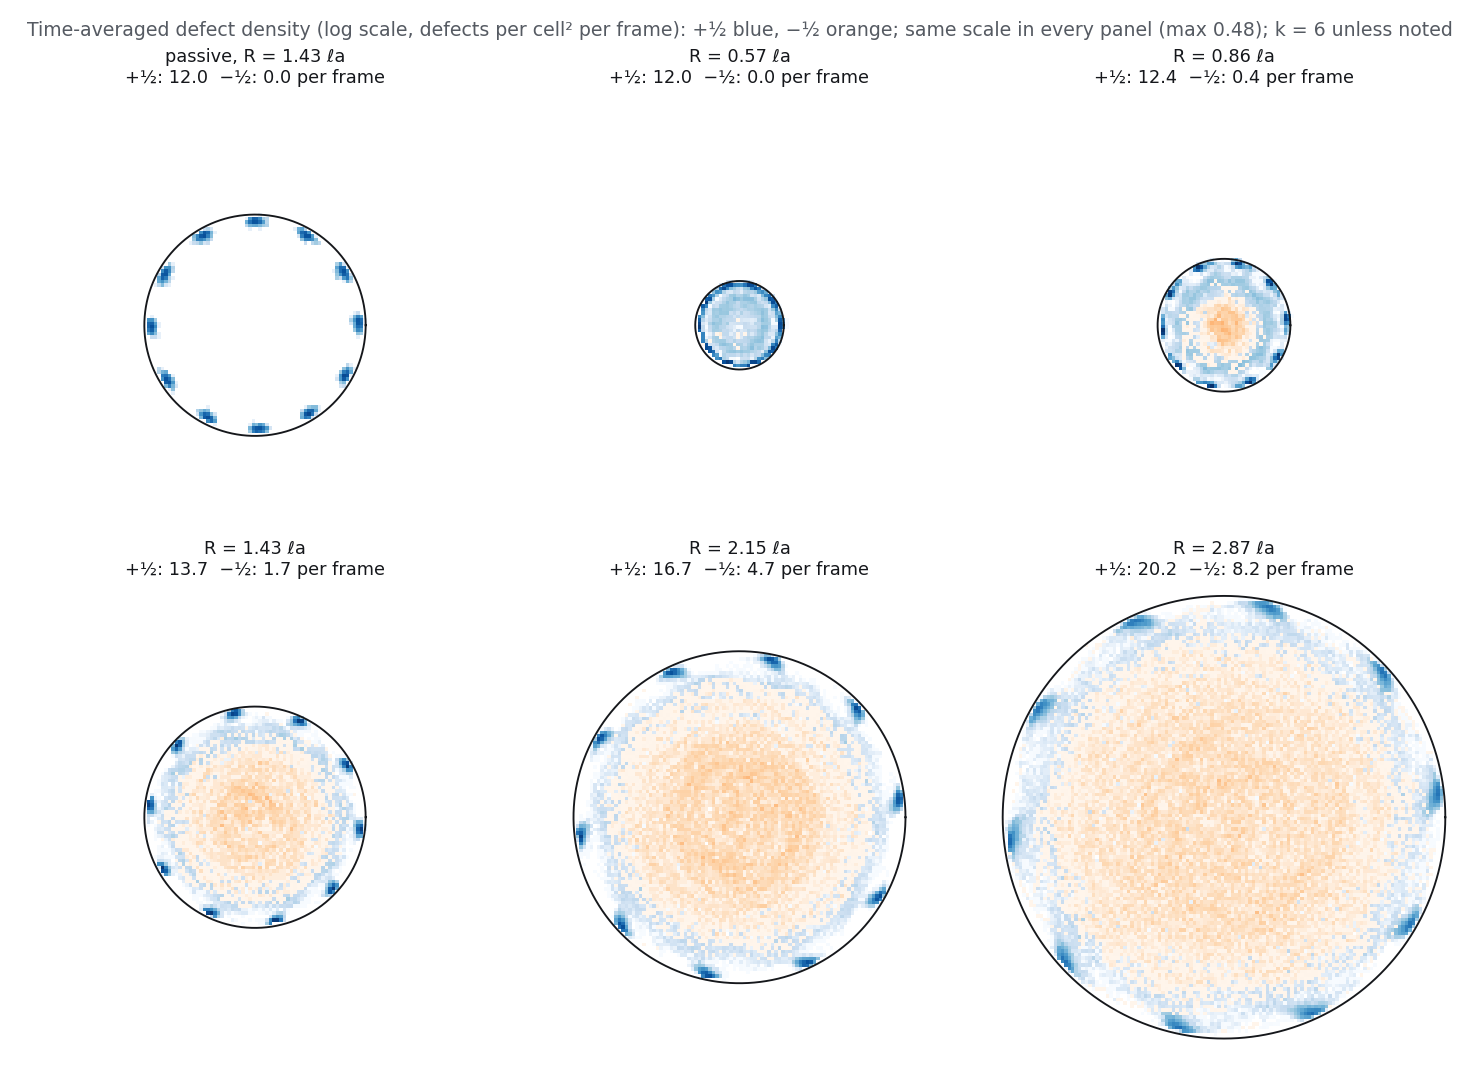
\includegraphics[width=0.92\textwidth]{maps_circles.png}
\caption{Time-averaged defect density, circles with $k=6$ (seed 1; log scale, the same scale in every panel; $+\half$ blue,
$-\half$ orange; per-frame counts in the panel titles, $N_+-N_-=2k=12$ in every run). Passive: 12 fixed spots at the wall.
$R=0.57\,\la$: no $-\half$, so no bulk; $\approx11$ of the 12 $+\half$ at the wall, already in a 10-site pattern but weakly
pinned, the 12th just inside. $0.86\,\la$: the first $\pm\half$ pairs (0.4 per frame); 10 $=2k-2$ wall sites. $1.43\,\la$: 10 pinned
sites, a ring of mobile $+\half$ just inside them, $-\half$ densest in the centre. $2.15$ and $2.87\,\la$: more pairs (4.7 and
8.2 per frame), $-\half$ spread over the whole inner half; the 10 sites persist, but at $2.87\,\la$ only $\approx7.6$ are occupied
at a time and the spots are elongated along the wall.}\label{fig:maps-circ}
\end{figure}

\begin{figure}[H]\centering
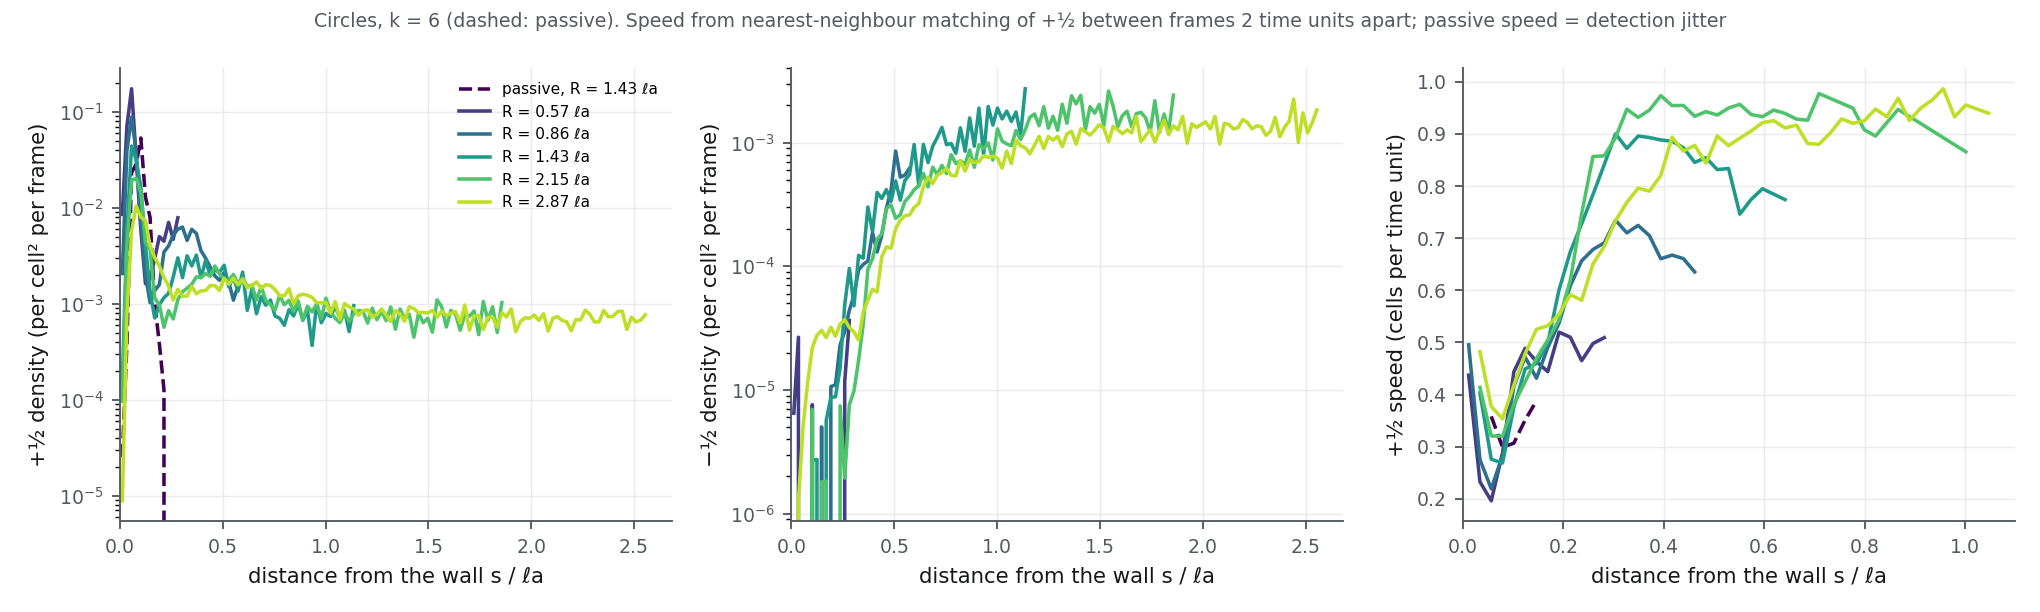
\includegraphics[width=\textwidth]{profiles_circles.png}
\caption{Circles, $k=6$: $+\half$ density, $-\half$ density and $+\half$ speed against the distance $s$ from the wall
(units of $\la$; dashed: passive). The $+\half$ density has a sharp wall peak at $s\approx1$--2 cells
($s/\la\approx0.05$--0.1), a depleted gap just inside it, and a flat bulk plateau ($\approx8\times10^{-4}$ per cell$^2$ per
frame, the same at every size). The $-\half$ are excluded from the outer $\approx0.3\,\la$ and uniform beyond $\approx0.7\,\la$.
Wall $+\half$ move at the passive jitter level (0.2--0.35 cells per time unit); the speed rises across the gap to
0.9--1.0 in the bulk of the larger cavities (lower in small cavities, where the bulk is close to the wall).}\label{fig:prof-circ}
\end{figure}

\begin{itemize}
  \item \textbf{Three zones.} A wall layer of pinned $+\half$ (peak at 1--2 cells), a gap at $s\approx3$--5 cells where both
        the density and the speed change, and a bulk of mobile $+\half$ and $-\half$ (structure below). The gap and the
        speed step sit at the same distance, which is what the density-minimum edge uses (Sec.~\ref{sec:edge}).
  \item \textbf{Size} (Fig.~\ref{fig:maps-circ}; numbers from the wall Fourier analysis, Sec.~\ref{sec:clattice}).
        At $0.57\,\la$ there are no bulk pairs: $\approx10.9$ $+\half$ are within the wall band, arranged with the 10-site
        ($2k-2$) period but only weakly pinned (static fraction 0.51, lattice memory 0.55); the remaining $+\half$ sits just
        inside. From $0.86\,\la$ pairs appear and the sites pin (static fraction 0.83 at 0.86, 0.99 at 1.43 and $2.15\,\la$).
        At $2.87\,\la$ the lattice still sits at fixed sites (lattice memory 0.97, static fraction 0.86) but is under-occupied,
        7.6 of 10 on average: the layer degrades by vacancies, not by sliding.
  \item \textbf{Bulk.} Up to $1.43\,\la$ the $-\half$ are densest in the centre ($3.5\times$ the density at $r/R=0.5$--0.75) and
        the bulk $+\half$ form a ring just inside the wall sites ($2.5\times$ the central density). In the larger cavities the
        $-\half$ fill the inner half uniformly; both signs are depleted only within $\approx0.3\,\la$ of the wall. Because the
        $-\half$ stay away from the wall, the accumulated charge $Q(r)$ dips below 0 inside before rising to the $+1$ plateau
        (Sec.~\ref{sec:ccharge}).
  \item The wall peak of the $+\half$ density falls with size (0.044 per cell$^2$ at $1.43\,\la$, 0.010 at $2.87\,\la$) mostly
        because the same $\approx10$ wall defects are spread along a longer wall; it is not by itself a sign of a weaker layer.
\end{itemize}

\subsection{Dependence on $k$ at fixed size}\label{sec:cdist-k}
\begin{figure}[H]\centering
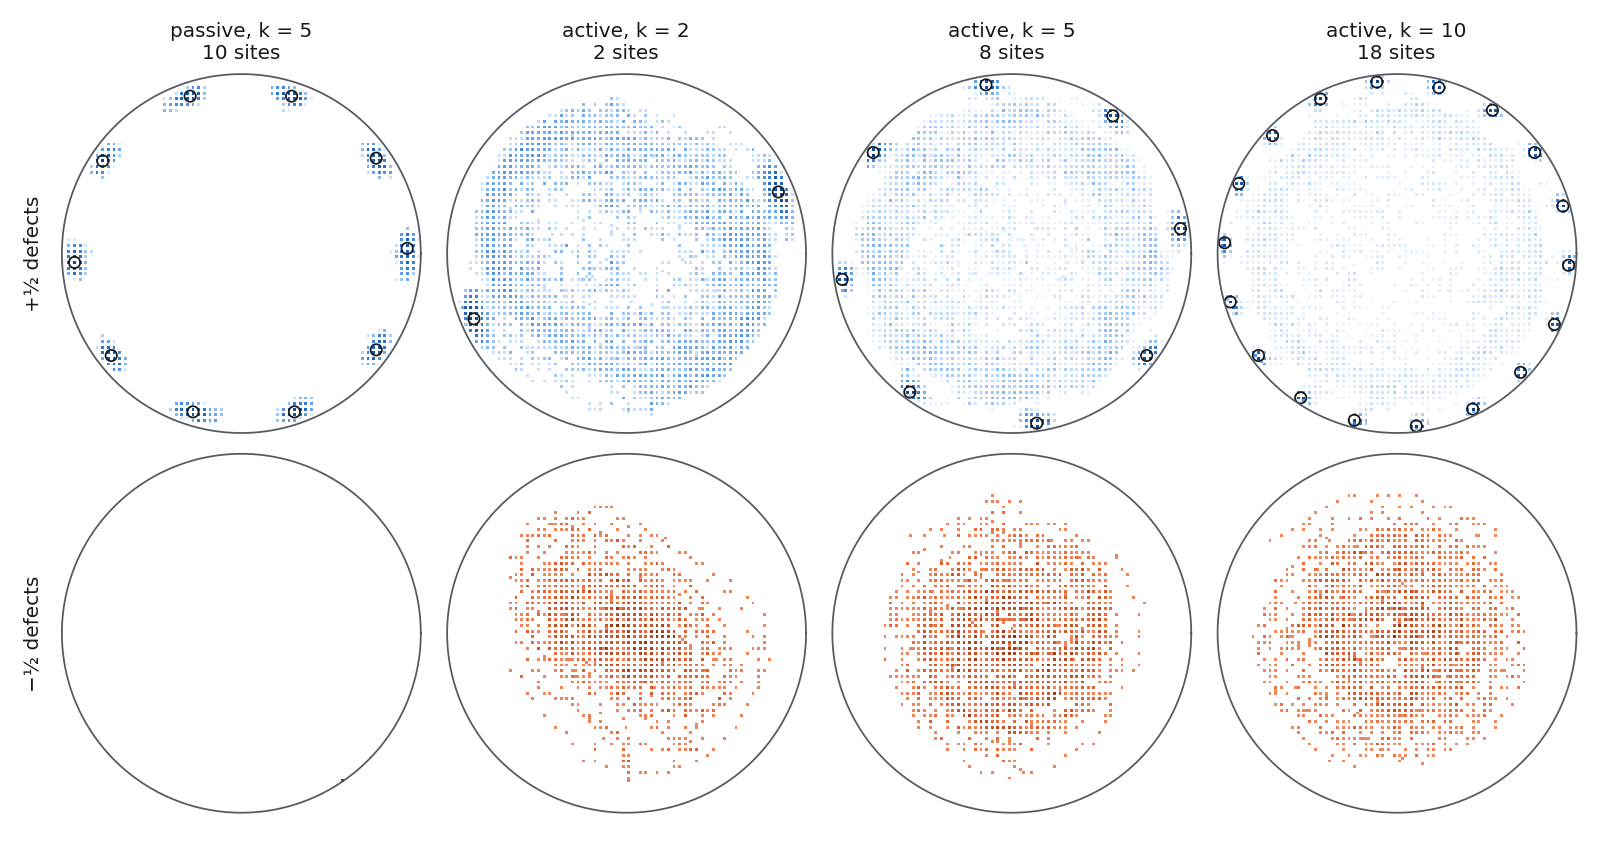
\includegraphics[width=\textwidth]{circle_maps_k.png}
\caption{Time-averaged density of $+\half$ (top) and $-\half$ (bottom), $R=1.43\,\la$: passive $k=5$ and active $k=2,5,10$
(seed 2). Open circles: pinned sites from the site rule, $2k$ passive and $2k-2$ active.}\label{fig:maps-k}
\end{figure}
\begin{figure}[H]\centering
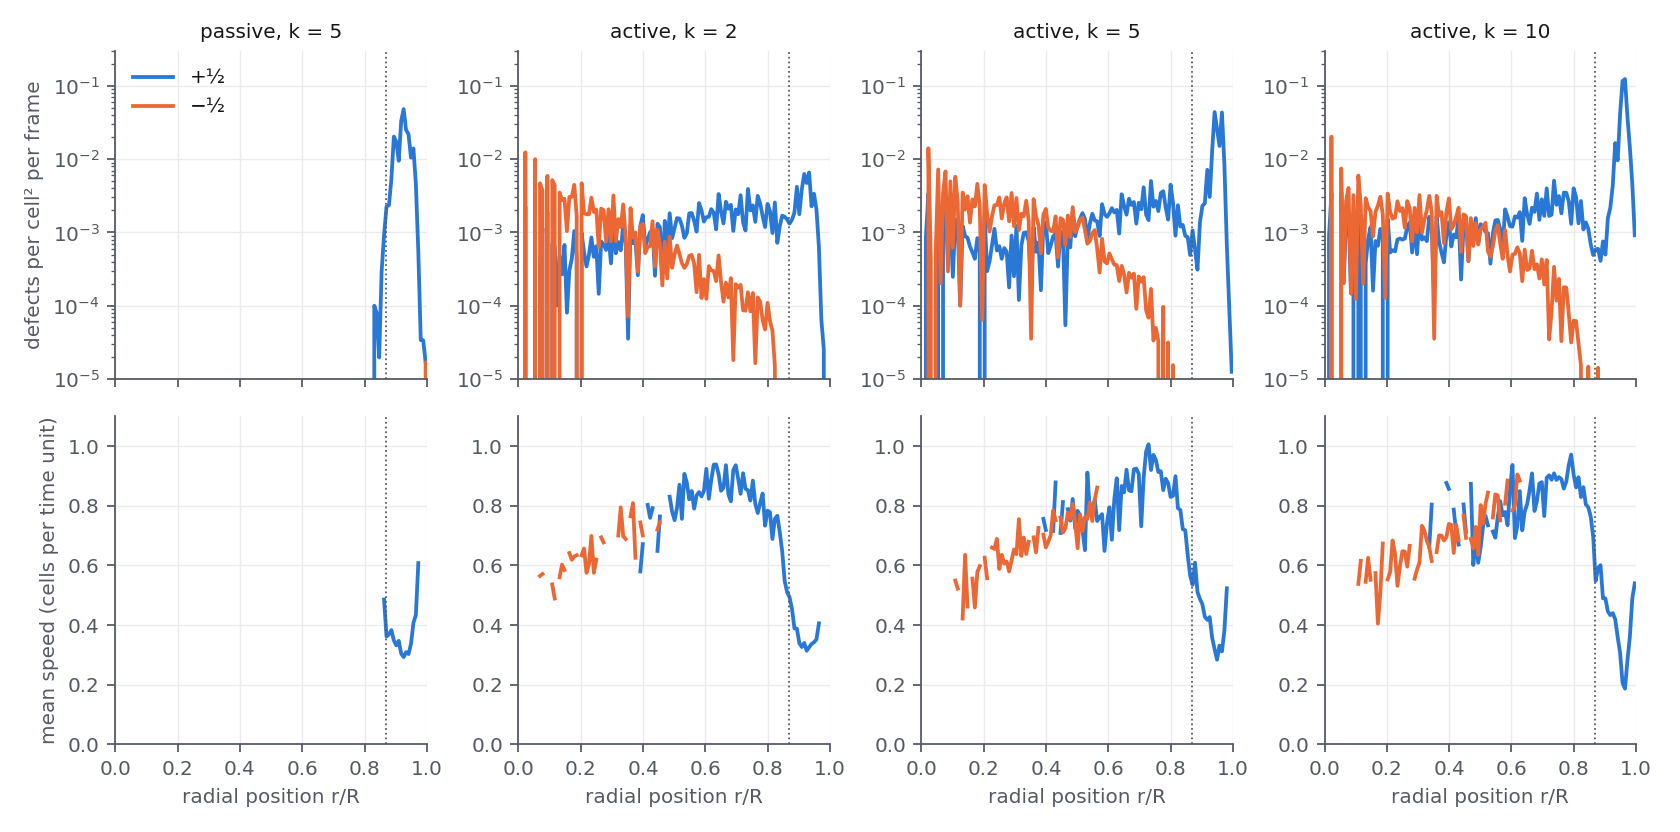
\includegraphics[width=\textwidth]{circle_radial.png}
\caption{Radial profiles at $R=1.43\,\la$ for the runs of Fig.~\ref{fig:maps-k}: $+\half$ and $-\half$ density and speed
against the distance from the wall.}\label{fig:radial-k}
\end{figure}
\begin{itemize}
  \item The number of wall sites is $2k-2$ in every active run of the fixed-radius scan (27/27 runs, $k=2\dots10$, 3 seeds),
        against $2k$ in the passive runs: two $+\half$ have left the wall to form the $+1$ bulk.
  \item The layer is diffuse and thicker at low $k$ and sharp at high $k$ (the spacing argument of Sec.~\ref{sec:passive}
        applies to the active layer too); the bulk is the same at every $k$.
  \item The capture distance of the site rule (minimum of the distance-to-nearest-site histogram, Fig.~\ref{fig:sitedist})
        shrinks with $k$ from 6.2 to 3.1 cells, about half the site spacing.
\end{itemize}
\begin{figure}[H]\centering
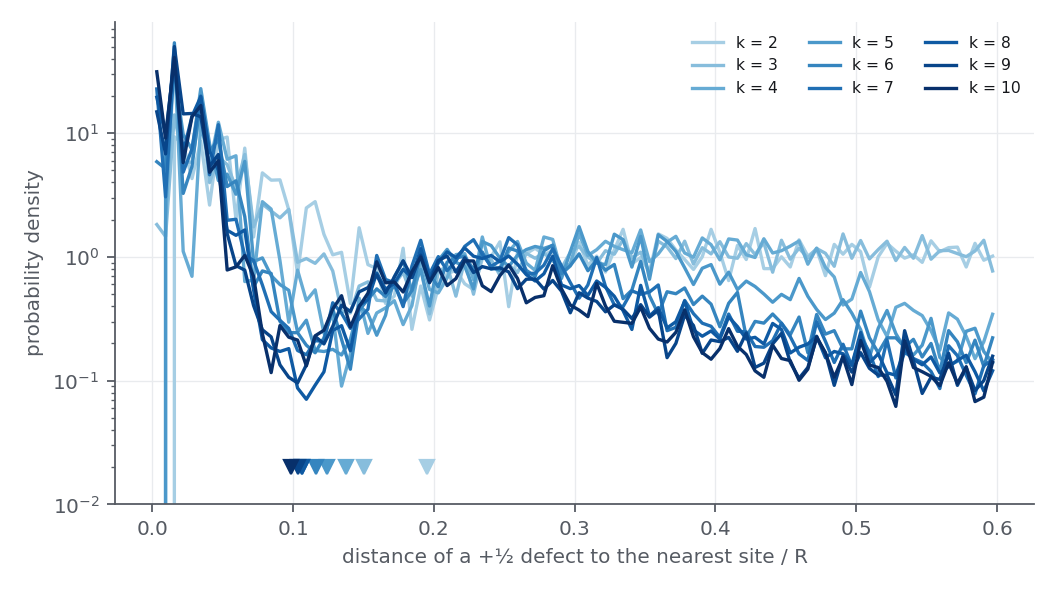
\includegraphics[width=0.85\textwidth]{circle_sitedist.png}
\caption{Distance of each $+\half$ to the nearest pinned site (histograms per run). The minimum separates defects on a
site (edge) from the rest (bulk) and defines the capture distance of the site rule.}\label{fig:sitedist}
\end{figure}

\subsection{Pair correlations}\label{sec:gr}
\SIcand
Ring-resolved pair correlations $g_{ab}(r\,|\,s)$ (reference defect binned by its distance $s$ from the wall, partner
anywhere, the radial profile divided out; method in Sec.~\ref{sec:m-gr}), pooled over $k$ and seeds of the fixed-radius scan.
\begin{figure}[H]\centering
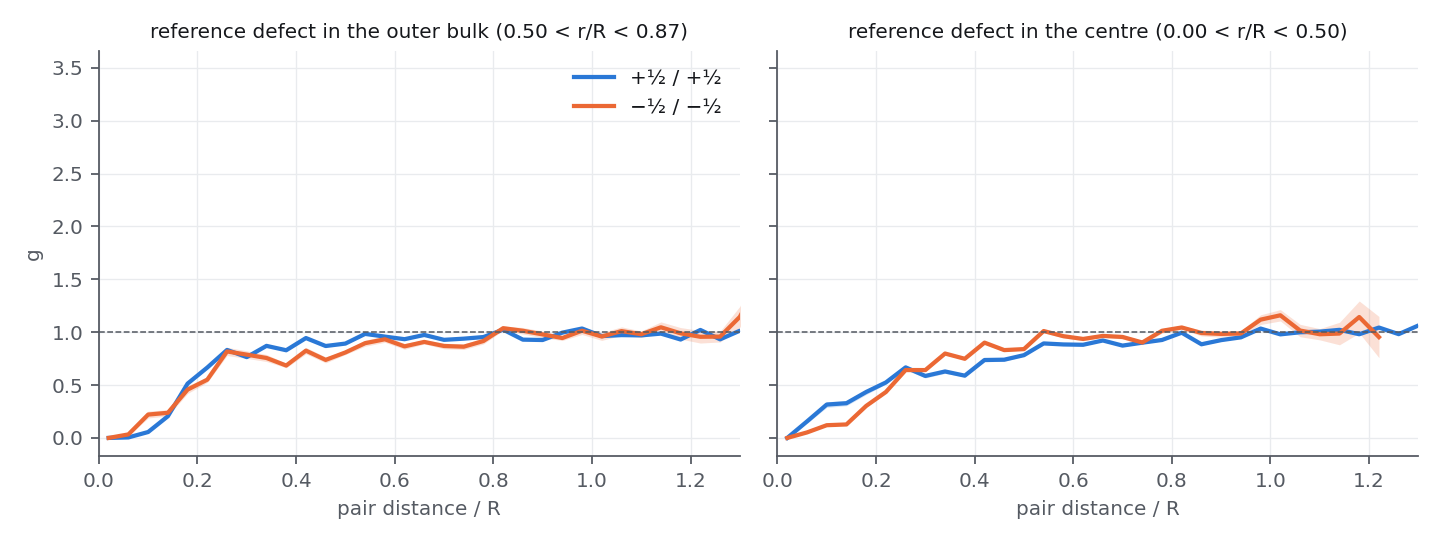
\includegraphics[width=0.49\textwidth]{g_same.png}\hfill
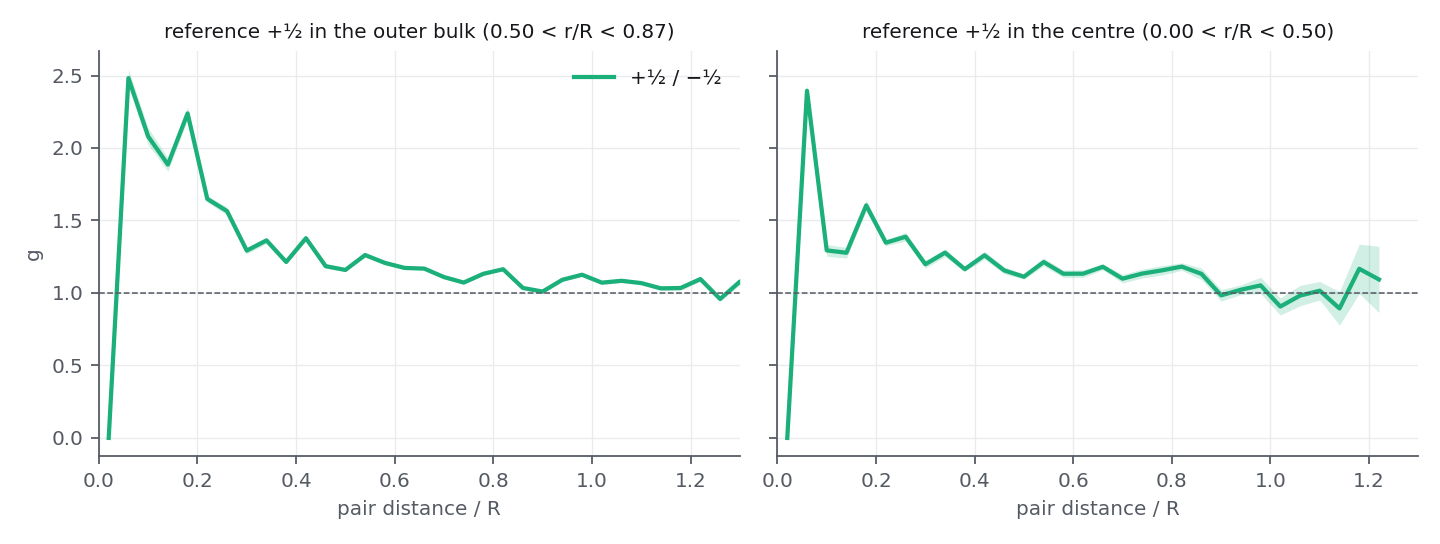
\includegraphics[width=0.49\textwidth]{g_pm.png}
\caption{Left: like-sign correlations $g_{++}$ (blue) and $g_{--}$ (orange) against the pair distance in units of $R$,
with the reference defect in the outer bulk ($0.5<r/R<0.87$) and in the centre ($r/R<0.5$); both have the same hole,
recovering to 1 at $\approx0.5$--$0.6R\approx\la$. Right: $g_{+-}$ for the same zones. $R=1.43\,\la$, pooled over
$k=2\dots10$ and 3 seeds; bands: Poisson error.}\label{fig:g}
\end{figure}
\begin{figure}[H]\centering
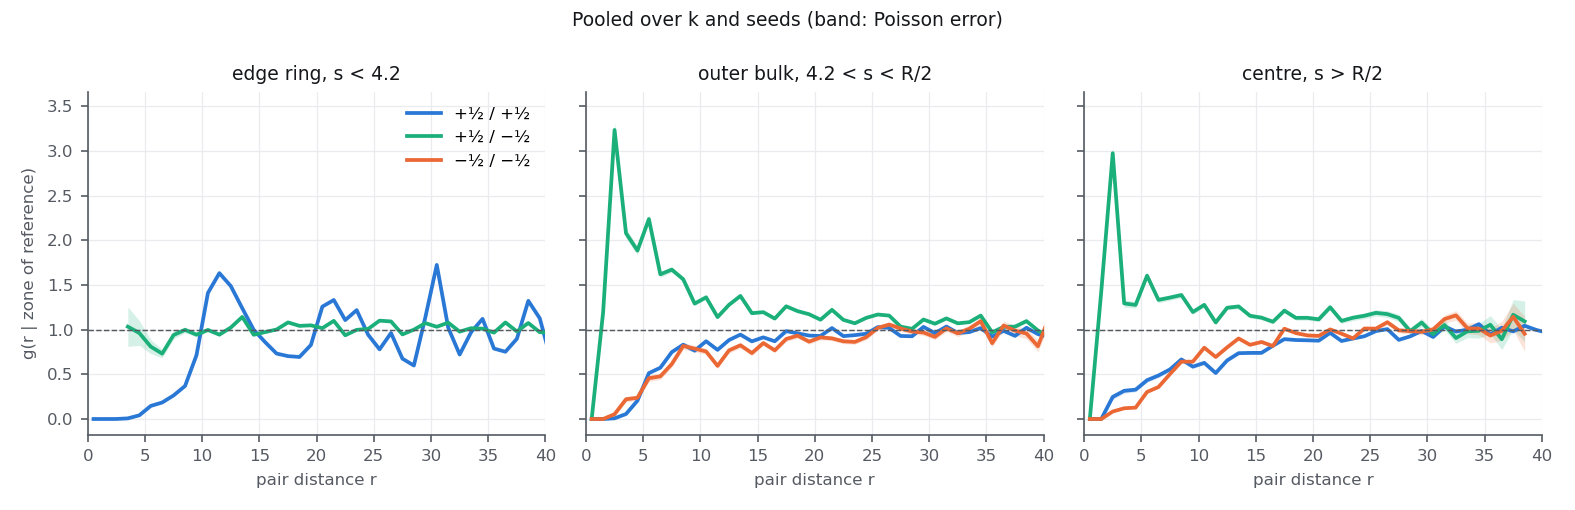
\includegraphics[width=0.9\textwidth]{g_zones.png}
\caption{Pooled $g(r\,|\,\text{zone})$ in cells, reference defect in the edge ring ($s<4.2$), the outer bulk
($4.2<s<R/2$) or the centre ($s>R/2$). Edge ring: $+\half/+\half$ lattice peaks at the site spacing ($\approx11$ cells
pooled over $k$) and its multiples; $+\half/-\half\approx1$. Bulk zones: $+\half/-\half$ peak $g\approx3$ at 2.5 cells;
like signs depleted below $\approx15$ cells.}\label{fig:gzones}
\end{figure}
\begin{itemize}
  \item \textbf{Bulk:} $+\half/-\half$ peak at $g\approx3.2$ at $r\approx2.5$ cells (fresh or annihilating pairs), with a tail
        above 1 out to 20--25 cells. Like signs have the same correlation hole: $g\approx0$ for $r<3$, 0.5 at $r\approx6$,
        1 at $r\approx15$--20 cells, i.e.\ about $\la$. The hole is slightly longer in the centre.
  \item \textbf{Wall ring:} $+\half/+\half$ lattice peak at the site spacing; $+\half/-\half\approx1$, so layer defects do
        not bind $-\half$.
  \item In units of $r/R$ ($\propto r/\la$ at fixed $R/\la$) the bulk $g_{++}$ collapses for $\zeta=0.05$, 0.07 and 0.09;
        $g_{--}$ collapses only up to $\approx0.5R$ at $\zeta=0.05$ (Sec.~\ref{sec:activity}).
  \item Known artefact: a red diagonal at the largest $r$ in the per-$k$ maps (partner in the far-side layer) comes from the
        thin layer peak in the expectation, not from a correlation.
\end{itemize}
